\documentclass[tikz, border=10pt]{standalone}
\usepackage{tikz}
\usetikzlibrary{arrows.meta}

\tikzset{
  cell/.style={draw, minimum width=0.9cm, minimum height=0.7cm,
               font=\small, align=center, inner sep=1pt},
  dead/.style={cell, fill=gray!20, text=gray},
  ptr/.style={-Stealth, semithick, shorten >=1pt},
}

\begin{document}
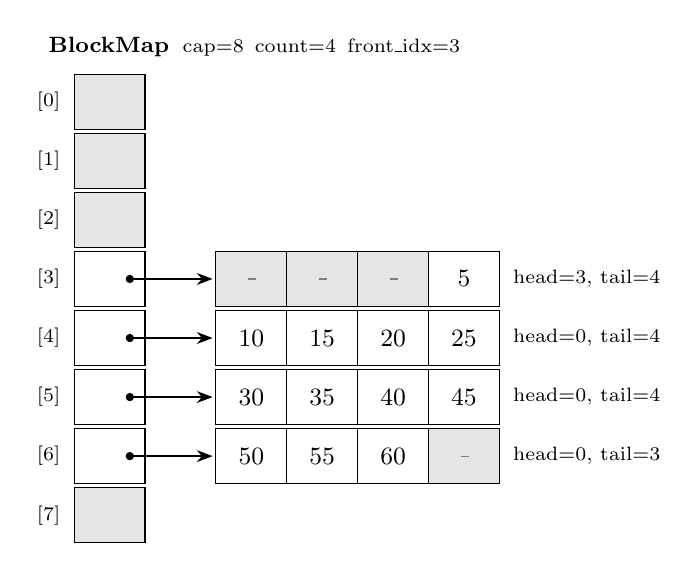
\begin{tikzpicture}[font=\small]

%% BlockMap
\node[anchor=south west, font=\footnotesize\bfseries] at (-0.9, 0.45)
  {BlockMap\enspace\normalfont\scriptsize cap=8\enspace count=4\enspace front\_idx=3};

% empty slots [0]–[2]
\foreach \i in {0,1,2} {
  \node[dead] (slot\i) at (0, {-\i*0.75}) {};
  \node[font=\scriptsize, anchor=east] at (-0.5, {-\i*0.75}) {[\i]};
}

% active slots [3]–[6]
\foreach \i in {3,4,5,6} {
  \node[cell] (slot\i) at (0, {-\i*0.75}) {};
  \node[font=\scriptsize, anchor=east] at (-0.5, {-\i*0.75}) {[\i]};
}

% empty slot [7]
\node[dead] (slot7) at (0, {-7*0.75}) {};
\node[font=\scriptsize, anchor=east] at (-0.5, {-7*0.75}) {[7]};

%% Block 0  head=3  tail=4  (1 element)
\node[dead] (b00) at (1.8, {-3*0.75}) {\_};
\node[dead]        at (2.7, {-3*0.75}) {\_};
\node[dead]        at (3.6, {-3*0.75}) {\_};
\node[cell]        at (4.5, {-3*0.75}) {5};
\node[font=\scriptsize, anchor=west] at (5.0, {-3*0.75})
  {head=3,\ tail=4};

%% Block 1  head=0  tail=4  (4 elements)
\node[cell] (b10) at (1.8, {-4*0.75}) {10};
\node[cell]        at (2.7, {-4*0.75}) {15};
\node[cell]        at (3.6, {-4*0.75}) {20};
\node[cell]        at (4.5, {-4*0.75}) {25};
\node[font=\scriptsize, anchor=west] at (5.0, {-4*0.75})
  {head=0,\ tail=4};

%% Block 2  head=0  tail=4  (4 elements)
\node[cell] (b20) at (1.8, {-5*0.75}) {30};
\node[cell]        at (2.7, {-5*0.75}) {35};
\node[cell]        at (3.6, {-5*0.75}) {40};
\node[cell]        at (4.5, {-5*0.75}) {45};
\node[font=\scriptsize, anchor=west] at (5.0, {-5*0.75})
  {head=0,\ tail=4};

%% Block 3  head=0  tail=3  (3 elements)
\node[cell] (b30) at (1.8, {-6*0.75}) {50};
\node[cell]        at (2.7, {-6*0.75}) {55};
\node[cell]        at (3.6, {-6*0.75}) {60};
\node[dead]        at (4.5, {-6*0.75}) {\_};
\node[font=\scriptsize, anchor=west] at (5.0, {-6*0.75})
  {head=0,\ tail=3};

%% Arrows: bullet inside slot, arrow to first block cell
\foreach \s/\t in {3/b00, 4/b10, 5/b20, 6/b30} {
  \coordinate (d\s) at ([xshift=-0.2cm]slot\s.east);
  \fill (d\s) circle (1.5pt);
  \draw[ptr] (d\s) -- (\t.west);
}

\end{tikzpicture}
\end{document}
